\section{Representation in latent space}
\begin{frame}{Transfer learning}
	\begin{center}
		\begin{figure}
			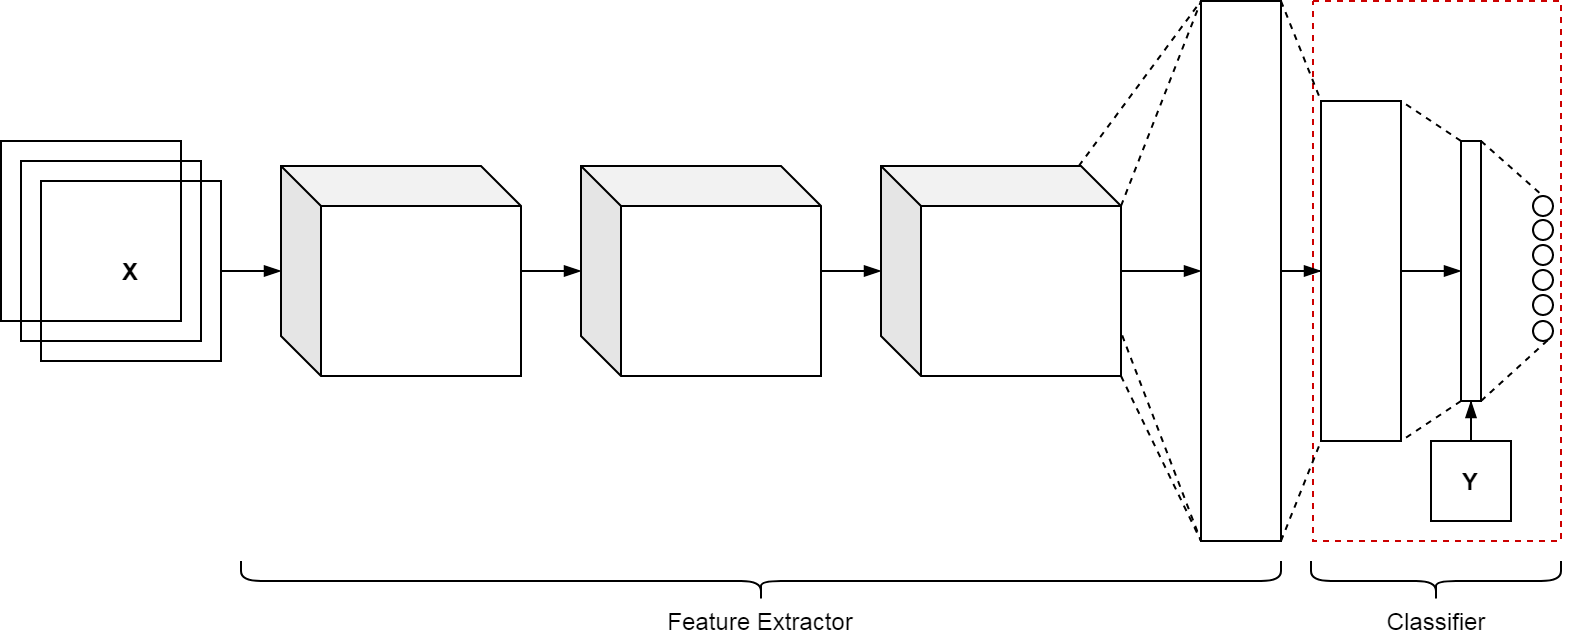
\includegraphics[width=1\textwidth]{figures/deep_cnn_transfer_learning_1}
		\end{figure}
	\end{center}
\end{frame}
\begin{frame}{Transfer learning}
	\begin{center}
		\begin{figure}
			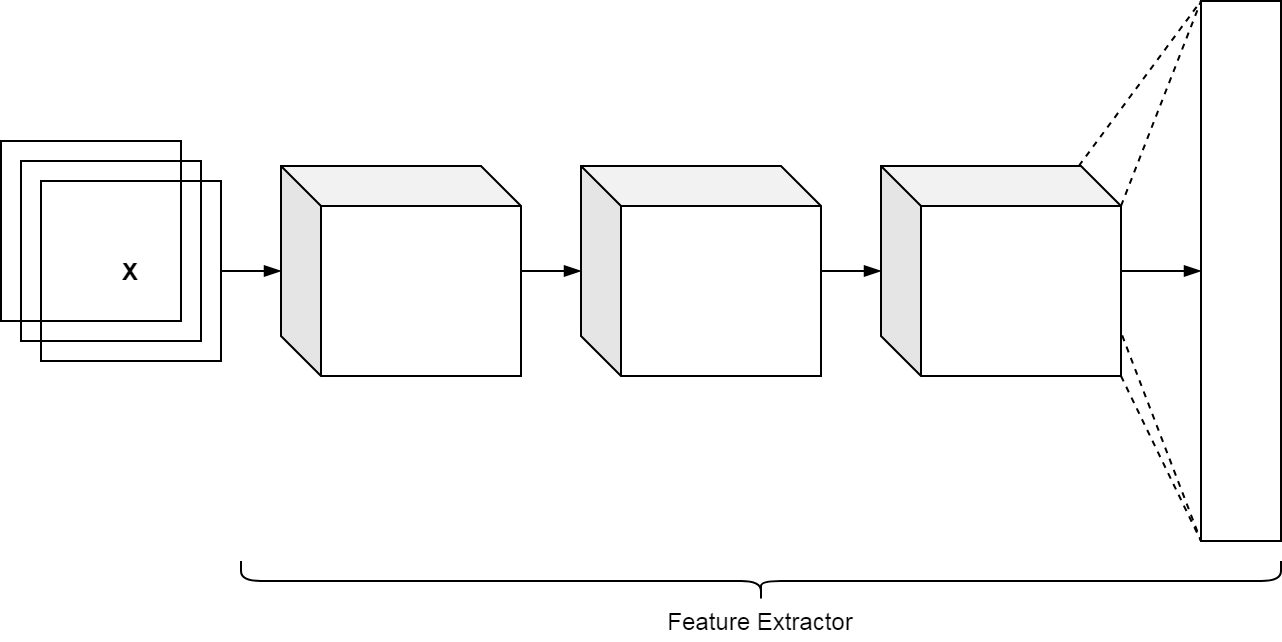
\includegraphics[width=1\textwidth]{figures/deep_cnn_transfer_learning_2}
		\end{figure}
	\end{center}
\end{frame}
\begin{frame}{Transfer learning}
	\begin{center}
		\begin{figure}
			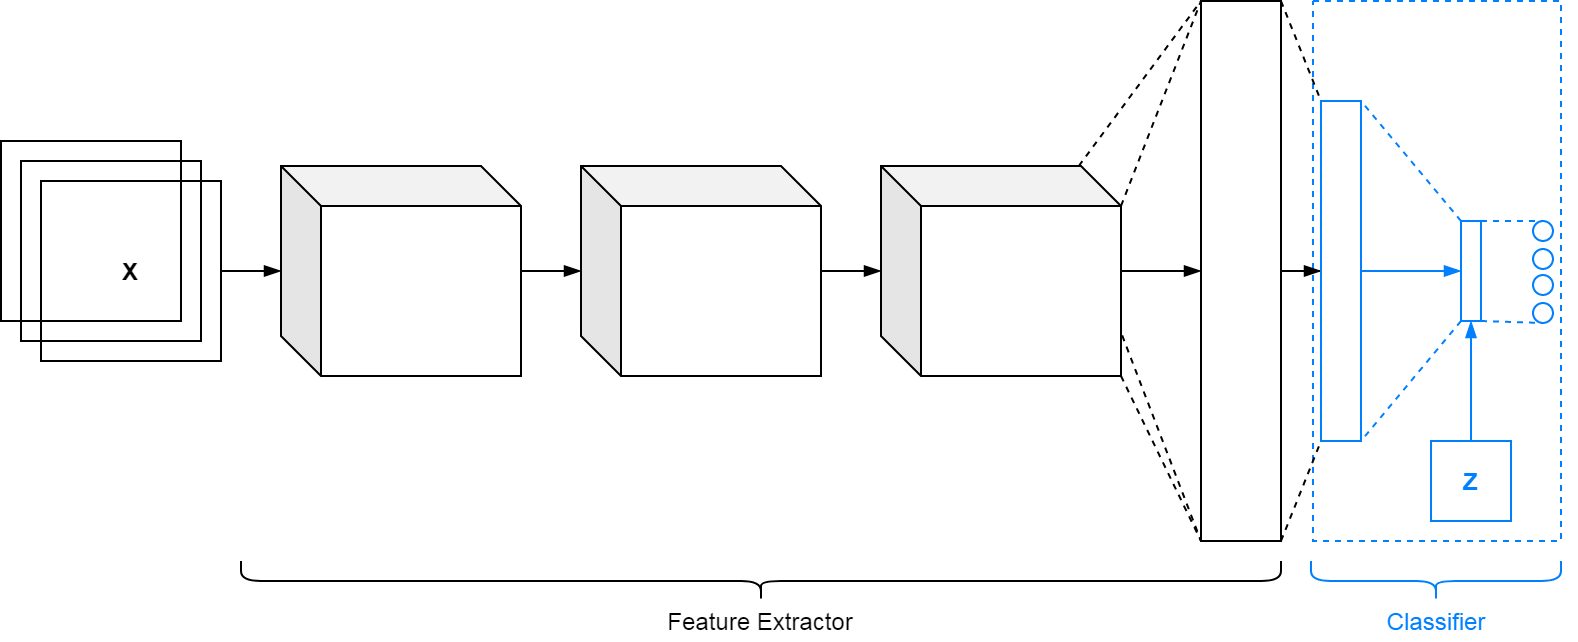
\includegraphics[width=1\textwidth]{figures/deep_cnn_transfer_learning_3}
		\end{figure}
	\end{center}
\end{frame}
\begin{frame}{Transfer learning - pytorch}
\begin{lstlisting}[language=Python,caption={Using pretrained ResNet18},captionpos=b]

import torch.nn as nn
from torchvision import datasets, models, transforms

model = models.resnet18(pretrained=True)
num_ftrs = model_ft.fc.in_features

# Here the size of each output sample is set to 2.
model.fc = nn.Linear(num_ftrs, 2)

\end{lstlisting}

\begin{lstlisting}[language=Python,caption={Freezing model parameters},captionpos=b]
for param in model.parameters():
  param.requires_grad = False
  
num_ftrs = model_ft.fc.in_features
model.fc = nn.Linear(num_ftrs, 2)
\end{lstlisting}

\end{frame}

\begin{frame}{Auto-encoders and approximate identity function}
\begin{itemize}
	\item Let us consider $y=f(x)$ as the network function.
	\item Let us consider another network function $y=g(x)$
	\item Let us consider a loss function, $L(x,g(f(x))$. This could be 
	\begin{itemize}
		\item[-] Mean squared distance 
		\item[-] Absolute difference 
		\item[-] "Some" other distance metric between vectors in "some" latent space 
	\end{itemize}  
\end{itemize}
	\begin{figure}
		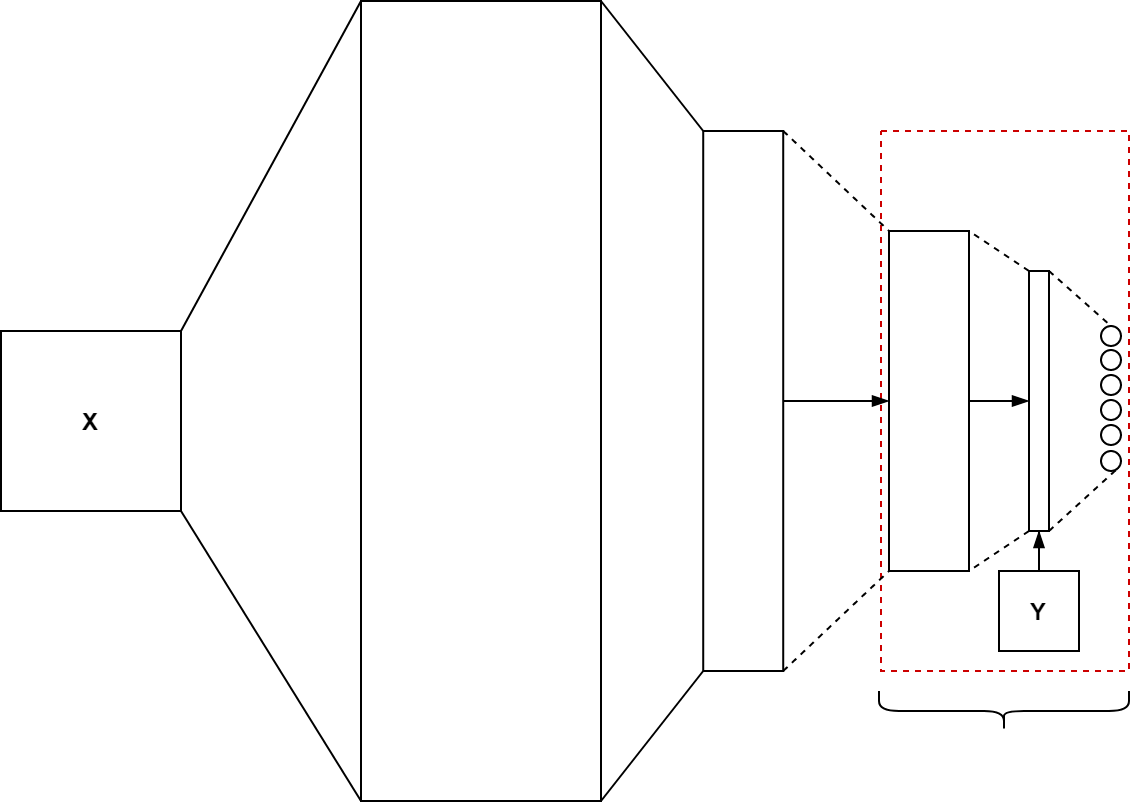
\includegraphics[width=.45\textwidth]{figures/autoencoder_1}
	\end{figure}
\end{frame}
\begin{frame}{Autoencoders and identity function} 
	\begin{center}
		\begin{figure}
			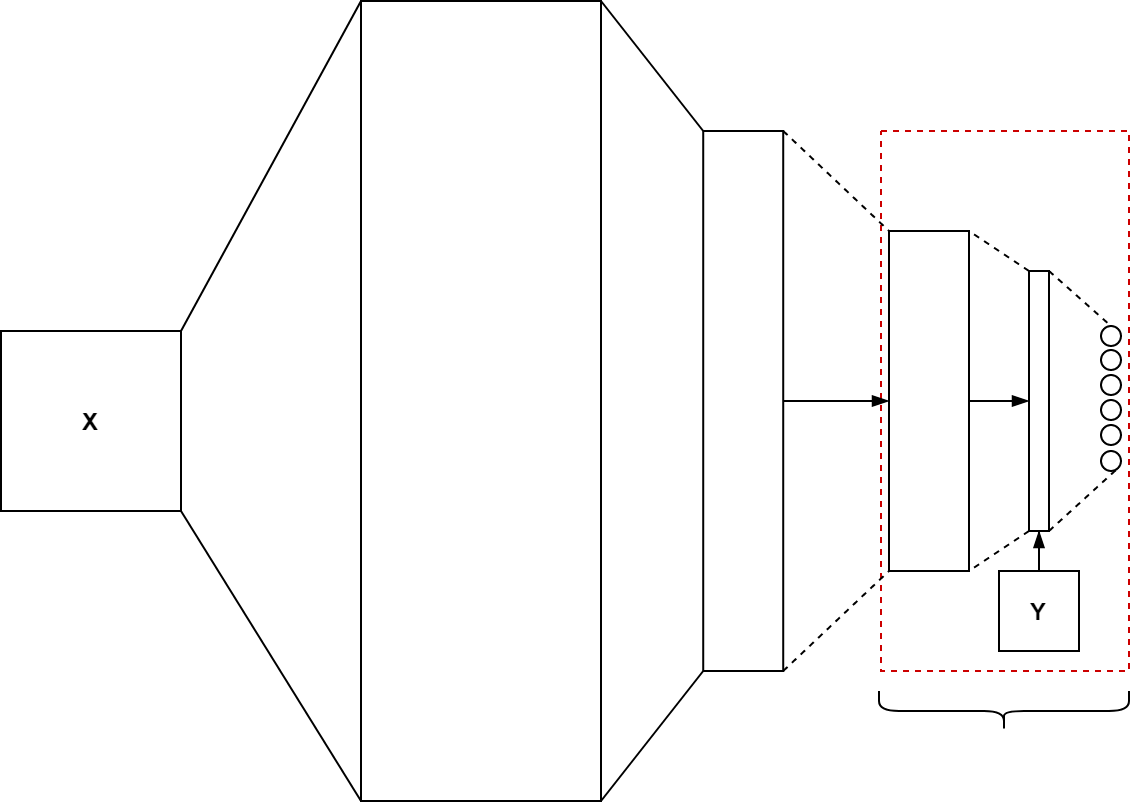
\includegraphics[width=.8\textwidth]{figures/autoencoder_1}
		\end{figure}
	\end{center}
\end{frame}
\begin{frame}{Autoencoders and identity function} 
	\begin{center}
		\begin{figure}
			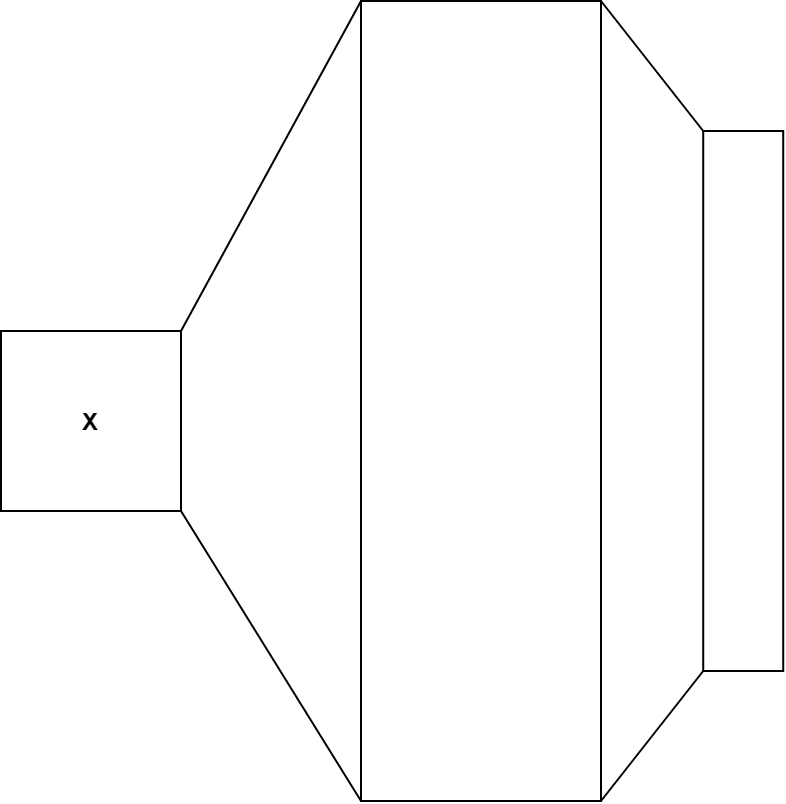
\includegraphics[width=.5\textwidth]{figures/autoencoder_2}
		\end{figure}
	\end{center}
\end{frame}
\begin{frame}{Autoencoders and identity function} 
	\begin{center}
		\begin{figure}
			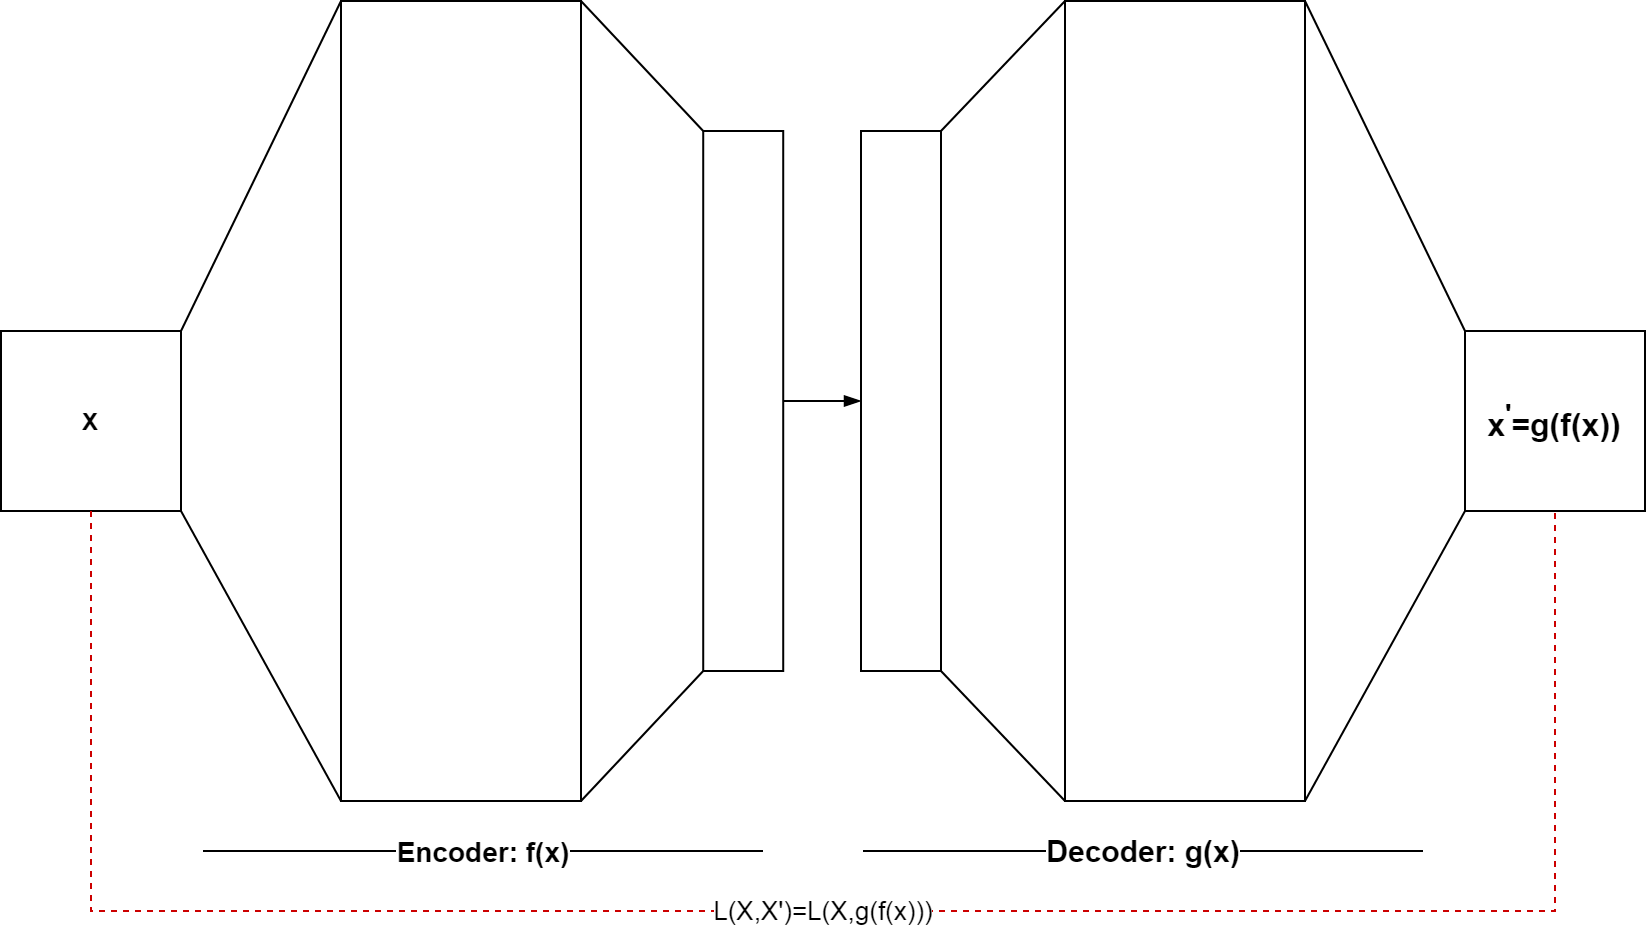
\includegraphics[width=.9\textwidth]{figures/autoencoder_3}
		\end{figure}
	\end{center}
\end{frame}
